\documentclass[10pt,a4paper]{article}

\usepackage[a4paper,hmargin=2.1cm,top=1.7cm,bottom=1.7cm]{geometry}
\usepackage[T1]{fontenc}
\usepackage{libertinus}
\usepackage{microtype}
\usepackage{array,booktabs,tabularx}
\usepackage[font=small,labelfont=bf,skip=5pt]{caption}
\usepackage{titlesec}
\usepackage{xcolor}
\usepackage{tikz}
\usetikzlibrary{positioning,fit,arrows.meta,calc}
\usepackage[hidelinks]{hyperref}

\definecolor{det}{HTML}{E8EEF4}
\definecolor{fit}{HTML}{FBE9D7}
\definecolor{acc}{HTML}{C96A00}
\definecolor{blu}{HTML}{1779A8}

\titleformat{\section}{\large\bfseries}{\thesection}{0.6em}{}
\titlespacing*{\section}{0pt}{12pt}{5pt}
\setlength{\parindent}{0pt}
\setlength{\parskip}{6pt}
\linespread{1.08}
\renewcommand{\arraystretch}{1.3}

\begin{document}

\begin{center}
{\Large\bfseries Predicting 90-Day Repeat Purchases from Transaction Histories}\\[8pt]
{\normalsize Group 41: Ludovico Piras, Nicolò Boscherini, Mattia Vannutelli}\\[2pt]
{\small Machine Learning 2026/27, NOVA IMS \textemdash{} Homework}
\end{center}

\begin{center}
\begin{minipage}{0.86\linewidth}
\small\textbf{Abstract.} We predict whether a customer purchases again within 90 days of a transaction. This handout outlines how we set up the workflow: a validation scheme that reproduces the temporal split between training and test data, rule-based cleaning, a preprocessing pipeline fitted within each fold, and L1-based feature selection. Our current model, a logistic regression with an F1-tuned threshold, reaches an F1 of 0.802 in validation and 0.804 on the Kaggle public leaderboard.
\end{minipage}
\end{center}

\section{Pipeline}

\begin{figure}[h]
\centering
\begin{tikzpicture}[
  font=\footnotesize, node distance=4mm and 5mm,
  box/.style={draw=black!50, rounded corners=2pt, align=center, minimum height=11mm, text width=24mm, inner sep=3pt, execute at begin node={\hyphenpenalty=10000\exhyphenpenalty=10000}},
  arr/.style={-{Stealth[length=2mm]}, black!65, thick}]
  \node[box, fill=det] (raw) {\textbf{Raw data}\\train 6,534 \textperiodcentered{} test 986};
  \node[box, fill=det, right=of raw] (clean) {\textbf{Cleaning}\\impossible values $\to$ NaN};
  \node[box, fill=det, right=of clean] (feat) {\textbf{Features}\\+ month, $-$ identifiers};
  \node[anchor=west, text=black!60, align=left, font=\footnotesize\itshape] at ($(feat.east)+(5mm,0)$) {fixed rules, identical\\for train and test};
  \node[box, fill=fit, below=11mm of raw] (imp) {\textbf{Impute}\\median / mode};
  \node[box, fill=fit, right=of imp] (scale) {\textbf{Transform}\\signed log, robust scaler};
  \node[box, fill=fit, right=of scale] (enc) {\textbf{Encode}\\one-hot, rare levels grouped};
  \node[box, fill=fit, right=of enc] (sel) {\textbf{Select}\\L1 logistic: 25 of 84};
  \node[box, fill=fit, right=of sel, text width=20mm] (mod) {\textbf{Model}\\logistic regression};
  \node[draw=acc, dashed, rounded corners=3pt, inner sep=2.5mm, fit=(imp)(mod)] (pipe) {};
  \node[anchor=south east, text=acc, font=\footnotesize\itshape] at (pipe.north east) {scikit-learn Pipeline, refitted in every fold};
  \node[box, below=10mm of sel, fill=white] (thr) {\textbf{Threshold 0.43}\\best out-of-fold F1};
  \node[box, below=10mm of mod, fill=white, text width=20mm] (out) {\textbf{Predictions}\\test IDs};
  \foreach \a/\b in {raw/clean, clean/feat, imp/scale, scale/enc, enc/sel, sel/mod, thr/out} \draw[arr] (\a) -- (\b);
  \draw[arr] (feat.south) -- ++(0,-3.5mm) -| (imp.north);
  \draw[arr] (mod.south) -- ++(0,-3mm) -| (thr.north);
\end{tikzpicture}
\caption{Overview of the pipeline. Grey steps apply fixed rules and learn nothing from the data; orange steps are fitted on training rows only.}
\end{figure}

\section{Validation strategy}

We started from how the test set relates to the training data. Test purchases begin 98 days after the last training purchase, each label depends on the following 90 days, and in 99.7\% of training rows the target coincides with the existence of a later row for the same customer. We therefore validate on three yearly blocks, training each fold only on purchases made at least 90 days before the block (Figure~\ref{fig:cv}), and we never derive features from a customer's later rows.

\begin{figure}[h]
\centering
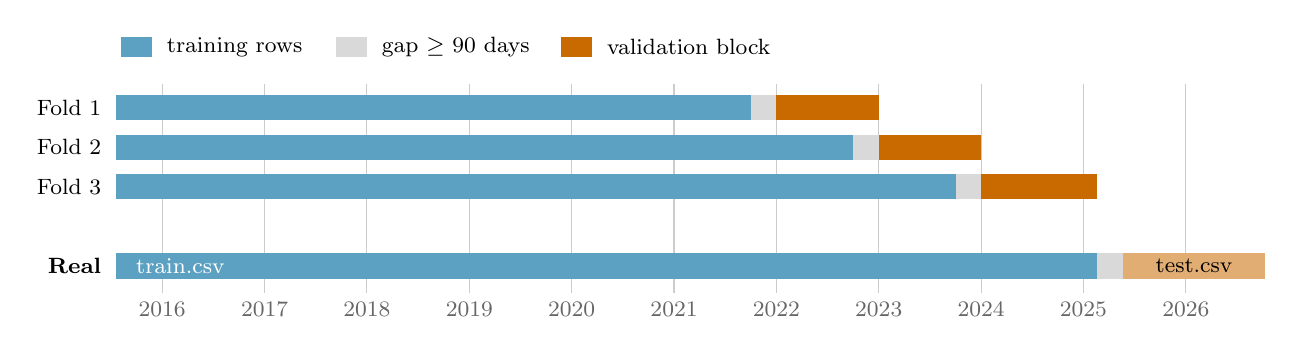
\begin{tikzpicture}[font=\footnotesize, x=1.3cm, y=5mm]
  \foreach \y in {2016,...,2026} \draw[black!20] ({\y-2015.5},0.6) -- ({\y-2015.5},-4.7) node[below, black!60] {\y};
  \newcommand{\fold}[5]{%
    \fill[blu!70] (0.05,-#1+0.32) rectangle ({#2-2015.5},-#1-0.32);
    \fill[black!15] ({#2-2015.5},-#1+0.32) rectangle ({#3-2015.5},-#1-0.32);
    \fill[acc] ({#3-2015.5},-#1+0.32) rectangle ({#4-2015.5},-#1-0.32);
    \node[anchor=east] at (0,-#1) {#5};}
  \fold{0}{2021.75}{2022.0}{2023.0}{Fold 1}
  \fold{1}{2022.75}{2023.0}{2024.0}{Fold 2}
  \fold{2}{2023.75}{2024.0}{2025.13}{Fold 3}
  \fill[blu!70] (0.05,-3.7) rectangle ({2025.13-2015.5},-4.34);
  \fill[black!15] ({2025.13-2015.5},-3.7) rectangle ({2025.39-2015.5},-4.34);
  \fill[acc!55] ({2025.39-2015.5},-3.7) rectangle ({2026.77-2015.5},-4.34);
  \node[anchor=east] at (0,-4.02) {\textbf{Real}};
  \node[anchor=west, text=white] at (0.15,-4.02) {train.csv};
  \node at ({2026.08-2015.5},-4.02) {test.csv};
  \fill[blu!70] (0.1,1.3) rectangle (0.4,1.8); \node[anchor=west] at (0.45,1.55) {training rows};
  \fill[black!15] (2.2,1.3) rectangle (2.5,1.8); \node[anchor=west] at (2.55,1.55) {gap $\geq$ 90 days};
  \fill[acc] (4.4,1.3) rectangle (4.7,1.8); \node[anchor=west] at (4.75,1.55) {validation block};
\end{tikzpicture}
\caption{Expanding-window cross-validation, designed to mirror the real split (bottom row).}\label{fig:cv}
\end{figure}

We preferred this scheme to random K-fold, which mixes past and future purchases. On our data the choice changes the conclusions: under random folds gradient boosting outperforms our model (ROC AUC 0.793 vs 0.790), while the time-ordered scheme reverses the ranking (0.774 vs 0.796). We did not use scikit-learn's \texttt{TimeSeriesSplit} either, as it splits rows into blocks of equal size and defines the gap in rows. Purchases are unevenly distributed over time, so this would produce arbitrary block boundaries and gaps of varying length. Splitting on calendar dates gives yearly blocks that cover the whole seasonal cycle and a gap of exactly 90 days.

We compare candidates on ROC AUC, which does not depend on the decision threshold, fold by fold, and adopt a change only when its gain is consistent across folds or supported by the exploration. Final choices rely on F1 for the positive class, against an all-positive baseline (0.753 on the last block). We select the decision threshold on the first two blocks and evaluate it on the third.

\section{Cleaning and pre-processing}

{\small
\begin{tabularx}{\linewidth}{@{}>{\raggedright\arraybackslash}p{3.6cm}>{\raggedright\arraybackslash}p{3.4cm}>{\raggedright\arraybackslash}X@{}}
\toprule
\textbf{Decision} & \textbf{Alternatives} & \textbf{Rationale} \\ \midrule
Remove 65 empty train rows & impute them & No information; source of all duplicates \\
Impossible values $\to$ NaN & row-by-row fixes & General rules (negative values, $10^9$ placeholder, inconsistent aggregates) \\
Median / mode imputation & mean, zero, KNN, iterative, missing indicators & Gaps are mostly structural (first purchases); all options within 0.004 ROC AUC \\
No outlier removal & drop extreme rows & Extremes are real large customers \\
Signed log, robust scaling & raw scale & Skewness up to 27; not applied to trees \\
One-hot, rare levels grouped & one column per level & 57 rare transport levels; unseen test levels \\
Add month of purchase & recency, trend, invoice ratios & Four-month repeat cycle; largest gain (+0.002) \\
No \texttt{clientes.csv} join (for now) & country, customer-since year & +0.001 in this form; revisited in Section 5 \\
\bottomrule
\end{tabularx}}

\section{Feature selection}

We did not discard identifier-like columns by default: we first checked whether they carry any signal. \texttt{ID} and \texttt{random\_noise} carry no signal on their own (ROC AUC 0.507 and 0.495), while \texttt{customer\_id} would let the model memorise individual customers and is kept only as a join key. Near-constant categoricals are left to the selection step.

We then compared variance and mutual-information filters, recursive feature elimination and an L1-penalised logistic regression, all refitted within each fold. Only L1 improved on every fold (Table~\ref{tab:sel}), keeping 25 of the 84 encoded columns, with a similar result for a weaker penalty. Its advantage comes from the many near-duplicate columns ($|\rho| \geq 0.9$), of which it retains one per group.

\begin{table}[h]
\centering\small
\renewcommand{\arraystretch}{1.2}
\begin{minipage}[t]{0.47\linewidth}\centering
\caption{Feature selection (logistic regression).}\label{tab:sel}
\begin{tabular}{@{}lcc@{}}
\toprule
Method & Columns & ROC AUC \\ \midrule
All features & 84 & 0.785 \\
Filter: variance & 77 & 0.786 \\
Filter: mutual information & 35 & 0.783 \\
Wrapper: RFE & 35 & 0.788 \\
\textbf{Embedded: L1} & \textbf{25} & \textbf{0.796} \\
\bottomrule
\end{tabular}
\end{minipage}\hfill
\begin{minipage}[t]{0.47\linewidth}\centering
\caption{Models at default settings.}\label{tab:models}
\begin{tabular}{@{}lcc@{}}
\toprule
Model & ROC AUC & F1 \\ \midrule
\textbf{Logistic regression + L1} & \textbf{0.796} & \textbf{0.802} \\
KNN ($k=25$) & 0.776 & 0.780 \\
Gradient boosting & 0.774 & 0.777 \\
Decision tree (depth 6) & 0.747 & 0.765 \\
\bottomrule
\end{tabular}
\end{minipage}
\end{table}


\section{Current results and next steps}

With the month of purchase and L1 selection, logistic regression outperforms the other models we tried at default settings (Table~\ref{tab:models}): its strongest inputs, recent purchase frequency and the usual gap between purchases, act almost monotonically on the target. The threshold of 0.43 maximises out-of-fold F1; it lies below 0.5 because, with 56\% of purchases being repeats, F1 rewards predicting the positive class more readily. With it the model reaches a validation F1 of 0.802, 0.049 above the all-positive baseline, and our submission scored 0.804 on the public leaderboard.

We are now working on two fronts. The first is hyperparameter tuning: the more flexible models are still at their default settings, and tuning will show whether they can match or improve on the linear model. The second is feature engineering with \texttt{clientes.csv}, which we did not integrate in the version presented here. Exploring the seasonal peaks, we found that purchases in peak months are not spread evenly across commercial regions. A feature that interacts the month of purchase with the customer's commercial region slightly improved our latest submission, and we are extending this idea to a geographic grouping of customers. Every such feature will be adopted only if it holds under the validation scheme of Section 2.

\end{document}
